%!TEX encoding = UTF-8 Unicode
%!TEX root = ../lect-w02.tex


\ifkompendium

\noindent Ett program innehåller satser och uttryck. En \Emph{kontrollstruktur}, t.ex. \code{while}, styr i vilken \Alert{ordning} satser och uttryck exekveras. Data kan placeras i en \Emph{datastruktur}, t.ex. en \code{Vector}, så att man senare kan komma åt data igen.    
\fi


\ifkompendium\else
\begin{SlideExtra}{Repetition: \texttt{val} \texttt{var} \texttt{def}}
  Vad är det för skillnad på (och likhet mellan) \code{val}, \code{var} och \code{def}? \pause
  \begin{itemize}
    \item Med \code{val} deklareras en variabel som tilldelas ett värde vid initialisering och som sedan \Emph{aldrig ändras}.
    \item Med \code{var} deklareras en variabel som tilldelas ett värde vid initialisering och som sedan \Alert{kan uppdateras} hur många gånger som helst med hjälp av tilldelningssatser.
    \item Med \code{def} deklareras en funktion som körs vid \Emph{varje anrop}
  \end{itemize}
  \pause\vspace{1em} En \Alert{konstighet i REPL}: 
  \begin{itemize}
  \item Man kan i REPL \Emph{deklarera} variabler och funktioner med \Emph{samma namn} \Alert{flera gånger} på samma nivå. 
  \item Detta ger i vanliga, fristående program \Emph{kompileringsfel}. 
  \end{itemize}
\end{SlideExtra}
\fi 

\Subsection{Datastrukturer}

\begin{Slide}{Vad är en datastruktur?}\SlideFontSmall
\begin{itemize}
\item En \href{https://sv.wikipedia.org/wiki/Datastruktur}{datastruktur} är en struktur för organisering av data som...
\begin{itemize}\SlideFontTiny
\item kan innehålla \Alert{många} element,
\item kan \Emph{refereras} till som en \Alert{helhet}, och
\item ger möjlighet att \Emph{komma åt} \Alert{enskilda element}.
\end{itemize}

\item En \Emph{samling} \Eng{collection} är en datastruktur som kan innehålla många element av \Alert{samma typ}.

\item Exempel på olika samlingar där elementen är organiserade på olika vis: \\
\vspace{0.5em}
\begin{tabular}{l c}
\Emph{Sekvens} & 
\includegraphics[width=5cm]{../img/list.pdf} \\
\Emph{Träd}  & 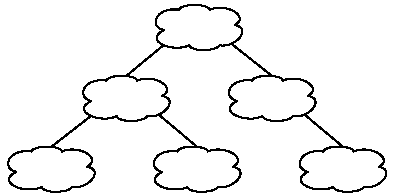
\includegraphics[width=2.2cm]{../img/tree.pdf} \\
\Emph{Graf}  & 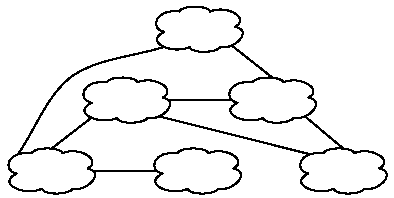
\includegraphics[width=2.2cm]{../img/graph.pdf} \\
\end{tabular}
\end{itemize}
{
\SlideFontTiny \vspace{1em }\hskip2em
Mer om sekvenser \& träd i \href{http://cs.lth.se/edaa01vt}{EDAA01 pfk}.
Mer om träd, grafer i \href{http://cs.lth.se/edaa40}{Diskreta strukturer.}
}

\end{Slide}

\begin{Slide}{Några samlingar i \texttt{scala.collection}}\SlideFontSmall
\SlideOnly{\setlength{\leftmargini}{0pt}}
\begin{itemize}
\item En \Emph{samling} \Eng{collection} är en datastruktur som kan innehålla många element av \Alert{samma typ}.
\item En \Emph{sekvens} \Eng{sequence} är en samling där alla element är ordnade.

\item Exempel på \Emph{färdiga samlingar} i Scalas standardbibliotek där elementen är organiserade  internt på \Alert{olika} vis så att samlingen får olika egenskaper som passar \Alert{olika användningsområden}:
\begin{itemize}\SlideFontTiny
\item \texttt{scala.collection.immutable.\Emph{Vector}}, sekvens med snabb access \Alert{överallt}.
\item \texttt{scala.collection.immutable.\Emph{List}}, sekvens med snabb access \Alert{i början}.
\item \texttt{scala.collection.immutable.\Emph{Set}}, \texttt{scala.collection.\Alert{mutable}.\Emph{Set}}, mängd med unika element; ej i sekvens men snabb innehållstest.
\item \texttt{scala.collection.immutable.\Emph{Map}}, \texttt{scala.collection.\Alert{mutable}.\Emph{Map}}, mängd med par av nyckel \& tillhörande värde, snabb access via nyckel.
\item \texttt{scala.collection.\Alert{mutable}.\Emph{ArrayBuffer}}, förändringsbar sekvens kan ändra storlek.
\item \texttt{scala.\Emph{Array}}, förändringsbar sekvens som \Alert{inte} kan ändra storlek. Alla element är lagrade efter varandra i minnet: snabbast access av alla samlingar, men har speciella begränsningar.
\end{itemize}
\end{itemize}
\end{Slide}


\begin{Slide}{Olika strukturer för att hantera data}
\begin{itemize}\SlideFontSmall
\item \Emph{Tupel} \Eng{tuple}
\begin{itemize}\SlideFontTiny
\item samla flera datavärden t.ex. \code{(1, "hej", true)} i element \Emph{\code{_1}}, \Emph{\code{_2}}, \Emph{\code{_3}} 
\item elementen kan vara av \Alert{olika} typ
\end{itemize}
\item \Emph{Enumeration} (även kallad \emph{uppräkning}) \Eng{enumeration}
\begin{itemize}\SlideFontTiny
\item Namnge uppräknade värden t.ex. \code+enum Color { case Red, Black }+
\item Värdena har ordningsnummer och är alla av \Alert{samma} typ (här \code{Color})
\end{itemize}
\item \Emph{Klass} \Eng{class}
\begin{itemize}\SlideFontTiny
\item samlar data i \Emph{attribut} med (väl valda!) namn
\item attributen kan vara av \Alert{olika} typ
\item definierar även \Emph{metoder} som använder attributen \\ (kallas även \Emph{operationer} på data)
\end{itemize}

\item \Emph{Färdig samling}
  \begin{itemize}
  \item speciella klasser som samlar data i element av \Alert{samma} typ
  \item exempel: \code{scala.collection.immutable.}\Emph{\code{Vector}}
  \item har ofta \emph{många} färdiga \Emph{bra-att-ha-metoder}, \\ se snabbreferensen \url{http://cs.lth.se/pgk/quickref}
  \end{itemize}

\item \Emph{Egenimplementerade samlingar}
  \begin{itemize}
  \item $\rightarrow$ fördjupningskurs
  \end{itemize}

\end{itemize}
\end{Slide}





\begin{Slide}{Vad är en vektor?}\SlideFontSmall
En \Emph{vektor}\footnote{Vektor kallas ibland på svenska även \href{https://sv.wikipedia.org/wiki/F\%C3\%A4lt_\%28datastruktur\%29}{fält}, men det skapar stor förvirring eftersom det engelska ordet \emph{field} ofta används för \emph{attribut} (förklaras senare).}
\Eng{vector} är en \Emph{sekvens} som är \Alert{snabb} att \Emph{indexera} i.
Åtkomst av element i en sekvens som t.ex. heter \code{xs} sker i Scala med \code{xs.apply(platsnummer)}:

\begin{REPL}
scala> val heltal = Vector(42, 13, -1, 0, 1)
val heltal: scala.collection.immutable.Vector[Int] = Vector(42, 13, -1, 0, 1)

scala> heltal.apply(0)   // platsnummer räknas från noll
val res0: Int = 42

scala> heltal(1)         // man kan i Scala skippa .apply före (
val res1: Int = 13

scala> heltal(5)         // ger körtidsfel då sjätte platsen inte finns
java.lang.IndexOutOfBoundsException: 5
  at scala.collection.immutable.Vector.checkRangeConvert(Vector.scala:132)
\end{REPL}
Utelämnar du \code{.apply} så skapar kompilatorn automatiskt ett anrop av \code{apply}.
\end{Slide}

\begin{Slide}{En konceptuell bild av en vektor}

\begin{REPLnonum}
scala> val heltal = Vector(42, 13, -1, 0, 1)

scala> heltal(0)
val res0: Int = 42
\end{REPLnonum}

\begin{tikzpicture}[font=\ttfamily]
\matrix [matrix of nodes, row sep=0, column 2/.style={nodes={rectangle,draw,minimum width=3em}}] (var) at (0cm, 2.8cm)
{
heltal   &  \makebox(16,12){ }\\
};
\matrix [matrix of nodes, draw=black,row sep=0, column 2/.style={nodes={rectangle,draw,minimum width=4em}}] (vec) at (4cm, 1cm)
{
\textit{plats} &  \\
0   &  \makebox(16,12){42}\\
1   &  \makebox(16,12){13}\\
2   &  \makebox(16,12){-1}\\
3   &  \makebox(16,12){0}\\
4   &  \makebox(16,12){1}\\
};
\filldraw[black] (0.7cm,2.8cm) circle (3pt) node[] (ref) {};
 \draw [arrow] (ref) -- (vec);
\end{tikzpicture}

%\vspace{1em} Elementen ligger på rad någonstans i minnet.
\end{Slide}



\begin{Slide}{En samling strängar}

\begin{itemize}
\item En vektor kan lagra \Emph{många} värden av samma typ.
\item Elementen kan vara till exempel heltal eller strängar.
\item Eller faktiskt vad som helst. (En s.k. \emph{generisk} samling.)
\end{itemize}

\begin{REPL}
scala> val grönsaker = Vector("gurka","tomat","paprika","selleri")
grönsaker: scala.collection.immutable.Vector[String] =
  Vector(gurka, tomat, paprika, selleri)

scala> val g = grönsaker(1)
val g: String = tomat

scala> val xs = Vector(42, "gurka", true, 42.0)
val xs: Vector[Matchable] = Vector(42, gurka, true, 42.0)
\end{REPL}
\SlideFontSmall Notera typen \code{Matchable} som betyder ''\Emph{nästan vilken typ som helst}''\\
%\footnote{
%(\code{Matchable} liknar \code{Object} i Java/C\# men är \Alert{mer generell}; 
(Mer om \code{Matchable} senare.)
%}
\end{Slide}



\Subsection{Kontrollstrukturer}


\begin{Slide}{Vad är en kontrollstruktur?}
\begin{itemize}
\item En \Emph{kontrollstruktur} påverkar i vilken ordning (sekvens) satser exekveras och uttryck evalueras.
\begin{itemize}
\item[] Exempel på \Emph{inbyggda} kontrollstrukturer:
\\\vspace{0.5em}\code{for}-\code{do}-sats \\ \code{while}-\code{do}-sats \\ \code{for}-\code{yield}-uttryck
\end{itemize}

\item[]

\item I Scala kan man definiera \Alert{egna} kontrollstrukturer.
\begin{itemize}
\item[] Exempel: \code{upprepa} som du använt i Kojo
\\\vspace{0.5em}\code|upprepa(4){fram; höger}|
\end{itemize}
\end{itemize}
\end{Slide}

\ifkompendium\else
\begin{SlideExtra}{Mitt första program: en oändlig loop på ABC80}
\begin{minipage}{0.8\textwidth}
\begin{verbatim}
10 print "hej"
20 goto 10
\end{verbatim}
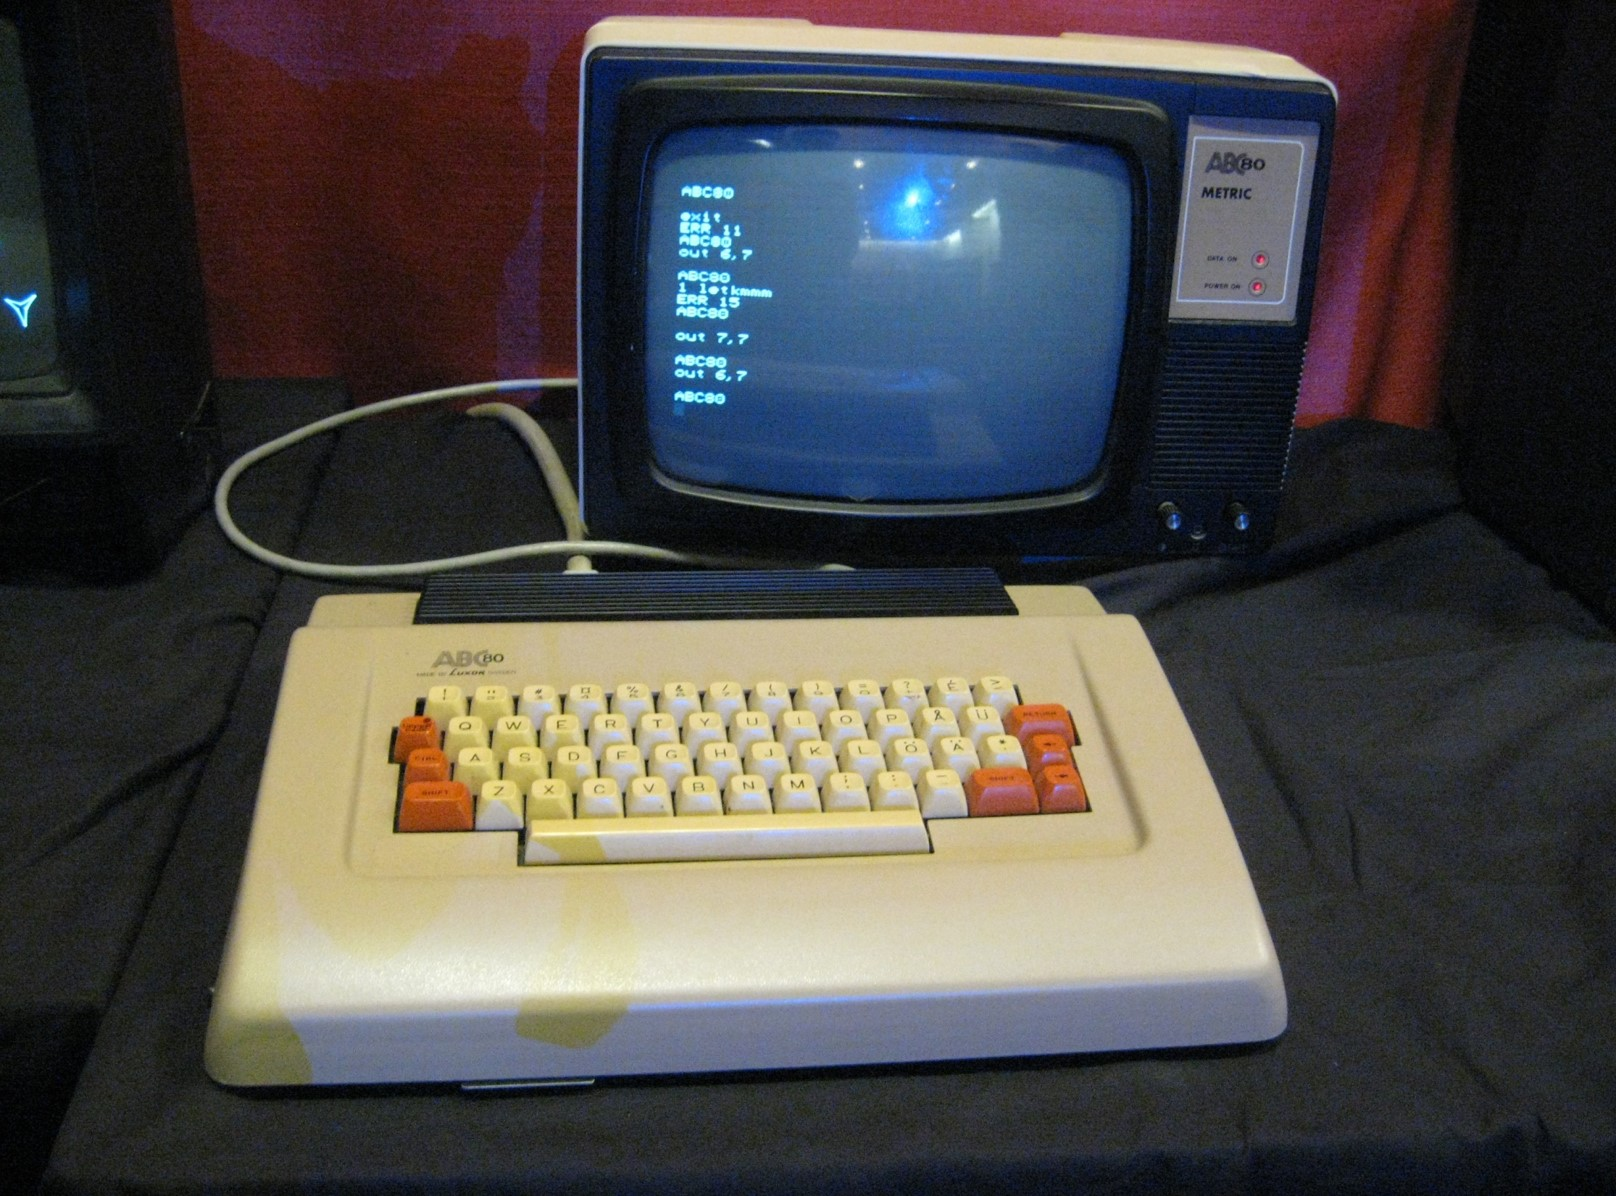
\includegraphics[width=0.8\textwidth]{../img/abc80.jpg}
\end{minipage}%
\begin{minipage}{0.2\textwidth}
\pause
\begin{verbatim}
hej
hej
hej
hej
hej
hej
hej
hej
hej
hej
hej
hej
<Ctrl+C>
\end{verbatim}
\end{minipage}
\end{SlideExtra}
\fi

\begin{Slide}{Loopa genom elementen i en vektor}
En \code{for}-\code{do}-\Emph{sats} som skriver ut alla element i en vektor:
\begin{REPL}
scala> val grönsaker = Vector("gurka","tomat","paprika","selleri")

scala> for g <- grönsaker do println(g)
gurka
tomat
paprika
selleri

\end{REPL}
\code{for ... do ...} gör så att följande händer:
\begin{itemize}
  \item Plocka ut \Emph{varje element} ur samlingen. 
  \item \Emph{Namnet} före pilen (här \code{g}) \Alert{refererar} till ett \Emph{nytt} värde för varje runda i loopen.
  \item Detta namn motsvarar en \Emph{lokal} \code{val}-variabel.
\end{itemize}
\end{Slide}


\begin{Slide}{Bygg ny samling från befintlig med for-yield-uttryck}
Ett \code{for}-\code{yield}-\Emph{uttryck} som \Emph{skapar en \Alert{ny} samling}.

\begin{Code}[basicstyle=\ttfamily\fontsize{12}{14}\selectfont]
for g <- grönsaker yield s"god $g"
\end{Code}

\begin{REPL}
scala> val grönsaker = Vector("gurka","tomat","paprika","selleri")

scala> val åsikter = for (g <- grönsaker) yield s"god $g"
val åsikter: Vector[String] =
  Vector(god gurka, god tomat, god paprika, god selleri)
\end{REPL}

\end{Slide}


\begin{Slide}{Samlingen \code{Range} håller reda på intervall}
\begin{itemize}
\item Med en \code{Range(start, slut)} kan du skapa ett \Emph{intervall}: \\ från och med \code{start} till (men inte med) \code{slut}
\end{itemize}

\begin{REPLnonum}
scala> Range(0, 42)
val res0: Range =
  Range(0, 1, 2, 3, 4, 5, 6, 7, 8, 9, 10, 11, 12, 13, 14,
    15, 16, 17, 18, 19, 20, 21, 22, 23, 24, 25, 26, 27, 28,
    29, 30, 31, 32, 33, 34, 35, 36, 37, 38, 39, 40, 41)
\end{REPLnonum}

\begin{itemize}
\item Men alla värden däremellan skapas inte förrän de behövs:
\end{itemize}

\begin{REPL}
scala> val jättestortIntervall = Range(0, Int.MaxValue)
val jättestortIntervall: Range = Range(0, 1, 2, 3, 4, 5, ...

scala> jättestortIntervall.end
val res1: Int = 2147483647

scala> jättestortIntervall.toVector
java.lang.OutOfMemoryError: GC overhead limit exceeded
\end{REPL}

\end{Slide}

\begin{Slide}{Loopa med Range}
\code{Range} används i for-loopar för att hålla reda på antalet rundor.
\begin{REPLnonum}
scala> for i <- Range(0, 6) do print(s" gurka $i")
 gurka 0 gurka 1 gurka 2 gurka 3 gurka 4 gurka 5
\end{REPLnonum}
Du kan skapa en \code{Range} med \code{until} efter ett heltal:
\begin{REPLnonum}
scala> 1 until 7
val res1: Range =
  Range(1, 2, 3, 4, 5, 6)

scala> for i <- 1 until 7 do print(s" tomat $i")
 tomat 1 tomat 2 tomat 3 tomat 4 tomat 5 tomat 6

\end{REPLnonum}
\end{Slide}

\begin{Slide}{Loopa med Range skapad med \texttt{to}}

Med \code{to} efter ett heltal får du en \code{Range} till och \Emph{med} sista:
\begin{REPLnonum}
scala> 1 to 6
res2: Range.Inclusive =
  Range(1, 2, 3, 4, 5, 6)

scala> for i <- 1 to 6 do print(" gurka " + i)
 gurka 1 gurka 2 gurka 3 gurka 4 gurka 5 gurka 6

\end{REPLnonum}


\end{Slide}



\begin{Slide}{Vad är en \code{Array}?}


\begin{itemize}
\item En \href{https://en.wikipedia.org/wiki/Array_data_structure}{\code{Array}} liknar en \code{Vector} men har en särställning i JVM:
\begin{itemize}
\item Lagras som en sekvens i minnet på efterföljande adresser.
\item \Emph{Fördel}: snabbaste samlingen för element-access i JVM.
\item Men det finns en hel del \Alert{nackdelar} som vi ska se senare.
\end{itemize}

\end{itemize}

\begin{REPLnonum}
scala> val heltal = Array(42, 13, -1, 0 , 1)
\end{REPLnonum}

\begin{tikzpicture}[font=\ttfamily,scale=0.75, every node/.style={scale=0.75}]
\matrix [matrix of nodes, row sep=0, column 2/.style={nodes={rectangle,draw,minimum width=3em}}] (var) at (0cm, 2.8cm)
{
heltal   &  \makebox(16,12){ }\\
};
\matrix [matrix of nodes, draw=black,row sep=0, column 2/.style={nodes={rectangle,draw,minimum width=4em}}] (vec) at (4cm, 1cm)
{
\textit{plats} &  \\
0   &  \makebox(16,12){42}\\
1   &  \makebox(16,12){13}\\
2   &  \makebox(16,12){-1}\\
3   &  \makebox(16,12){0}\\
4   &  \makebox(16,12){1}\\
};
\filldraw[black] (0.7cm,2.8cm) circle (3pt) node[] (ref) {};
 \draw [arrow] (ref) -- (vec);
\end{tikzpicture}
\end{Slide}

\begin{Slide}{Några likheter \& skillnader mellan \texttt{Vector} och \texttt{Array}}\SlideFontSmall
\begin{multicols}{2}
\begin{REPLnonum}
scala> val xs = Vector(1,2,3)
\end{REPLnonum}

\columnbreak

\begin{REPLnonum}
scala> val xs = Array(1,2,3)
\end{REPLnonum}
\end{multicols}


Några likheter mellan \texttt{Vector} och \texttt{Array}
\begin{itemize}
\item Båda är samlingar som kan innehålla många element.

\item Med båda kan man snabbt accessa vilket element som helst: \code{xs(2)}
\end{itemize}
Några viktiga skillnader:

\vspace{-0.5em}\begin{multicols}{2}
\Emph{Vector}
\begin{itemize}
\item Är \Emph{oföränderlig}: du kan lita på att elementreferenserna aldrig någonsin kommer att ändras.

\item Är \Emph{snabb på att skapa en delvis förändrad kopia}, t.ex. tillägg/borttagning/uppdatering mitt i sekvensen.

\end{itemize}


\columnbreak

\Alert{Array}
\begin{itemize}
\item Är \Alert{föränderlig}: \code{xs(2) = 42}

\item Är \Alert{snabb} om man bara vill läsa eller skriva på befintliga platser.

\item Är \Alert{långsam} om man vill lägga till eller ta bort element mitt i sekvensen.
\item Kan \Alert{ej} ändra storlek.

\end{itemize}
\end{multicols}
\end{Slide}



\Subsection{Fristående applikation}

\ifkompendium\else
\begin{SlideExtra}{Kompilering i terminalen}
  Nu ska du en skriva kod i en editor, kompilera i terminalen och köra ditt program som en \Emph{fristående applikation}. Då behövs:
  \begin{itemize}
    \item En editor, \Emph{VS Code} rekommenderas
    \item Körmiljön \Emph{OpenJDK} 
    \item Scala-kompilatorn: direkt med \Alert{\texttt{scalac}} eller via \code{scala-cli}
    \item Se instruktioner här: \url{http://cs.lth.se/pgk/verktyg}
    \item Tips om du kör Windows: installera %\href{https://docs.microsoft.com/en-us/windows/terminal/get-started}
    {nya Windows Terminal}

  \end{itemize}
    Be om hjälp i \texttt{\#frågor-och-svar}-textkanalen på vår Discord-server eller fråga handledare på resurstid.
  
\end{SlideExtra}
\fi

\begin{Slide}{Ett minimalt fristående program i Scala}\SlideFontSmall
Spara nedan Scala-kod i filen \code{hej.scala}:
\begin{Code}
@main def run = println("Hej Scala!")
\end{Code}

Spara i filen \code{hej.scala}, kompilera och kör i terminalen:
\begin{REPL}
> cat hej.scala
@main def run = println("Hej Scala!")

> scalac hej.scala

> ls
'hej$package.class'  'hej$package$.class'  'hej$package.tasty'   
hej.scala   run.class   run.tasty

> scala run 
Hej Scala! 
\end{REPL}

\end{Slide}


\begin{Slide}{Loopa genom en samling med en \texttt{while}-sats}
\begin{REPLnonum}
scala> val xs = Vector("Hej","på","dej","!!!")
val xs: Vector[String] =
  Vector(Hej, på, dej, !!!)

scala> xs.size
val res0: Int = 4

scala> var i = 0
val i: Int = 0

scala> while i < xs.size do { println(xs(i)); i = i + 1 }
Hej
på
dej
!!!
\end{REPLnonum}
\end{Slide}


\begin{Slide}{Strängargument till i ett program med primitiv main}
Skriv och spara nedan kod i filen \texttt{helloargs1scala}
\begin{REPLnonum}
> code helloargs1.scala
\end{REPLnonum}
\begin{Code}
object HelloScalaArgs:
  def main(args: Array[String]): Unit = // en primitiv main-metod utan @main
    var i = 0
    while i < args.size do
      println(args(i))
      i = i + 1
\end{Code}
En primitiv \code{main}-metod har ej \code{@main} och måste vara i ett objekt. \\
Kompilera och kör med namnet på objektet:
\begin{REPL}
> scalac helloargs1.scala
> scala HelloScalaArgs morot gurka tomat
morot
gurka
tomat
\end{REPL}
\end{Slide}

\begin{Slide}{Typsäkra argument till i ett program med @main}
  \SlideFontSmall
Skriv och spara nedan kod i filen \texttt{helloargs2.scala}
\begin{REPLnonum}
> code helloargs2.scala
\end{REPLnonum}
\begin{Code}
@main def hej(heltal: Int, resten: String*): Unit = 
  for i <- 0 until heltal do println(resten(i))
\end{Code}
Med \code{@main} behövs inget objekt.\\
Kompilera och kör med namnet på \code{@main}-funktionen:
\begin{REPL}
> scalac helloargs2.scala
> scala hej 2 morot gurka tomat
morot
gurka
> scala hej aj morot gurka tomat
Illegal command line: java.lang.NumberFormatException: For input string: "aj"
\end{REPL}
Med \code{@main} genereras automatiskt en primitiv main som kollar att argumenten har rätt typ.
\end{Slide}


\begin{Slide}{För kännedom: Scala-\textbf{skript}}
\begin{itemize}
  \item 
\SlideFontSmall
Scala-kod kan köras som ett \Emph{skript}.\footnote{\SlideFontTiny Vi kommer inte använda skript i kursen, som tyvärr ej kan inkludera flera kodfiler.
}
Ett skript kompileras varje gång innan det körs och maskinkoden sparas \emph{inte} som vid vanlig kompilering. 

\begin{Code}
// spara detta i filen 'myscript.scala'
@main def Huvudprogram(args: String*) =
  println("Hej alla mina argument:")
  for arg <- args do println("Hej: " + arg)
\end{Code}
Inkludera \code{.scala} i filnamnet om du vill köra som skript.  
\begin{REPLnonum}
> scala myscript.scala ett två tre
\end{REPLnonum}
\item
Det är lätt hänt att av misstag skriva \code{scala Huvudprogram.scala}, när du egentligen vill köra ett redan kompilerat program. Då ska \emph{inte} filändelsen \code{.scala} anges.
\end{itemize}
\end{Slide}



\Subsection{Algoritmer: stegvisa lösningar}

\begin{Slide}{Vad är en algoritm?}
En \href{https://sv.wikipedia.org/wiki/Algoritm}{algoritm} är en sekvens av instruktioner som beskriver hur man löser ett problem.

\vspace{1em}\Emph{Exempel}:
\begin{itemize}
\item	 baka en kaka
\pause\item räkna ut din pensionsprognos
\pause\item köra bil
\pause\item kolla om highscore i ett spel
\end{itemize}
\ifkompendium\else
\begin{tikzpicture}[overlay]
\node[xshift=0.85\textwidth, scale=2.0] { 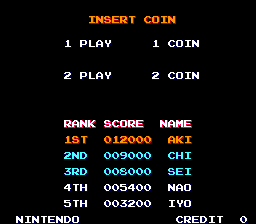
\includegraphics[width=0.25\textwidth]{../img/highscore}};
\end{tikzpicture}
\fi
\end{Slide}


\ifkompendium\else
\begin{SlideExtra}{Algoritm-exempel: HIGHSCORE}
\Emph{Problem}: Kolla om high-score i ett spel \\ \vspace{1em}

\Emph{Varför?} \pause Så att de som spelar uppmuntras att spela mer :) \\ \vspace{1em}

\Emph{Algoritm:}\pause
\begin{enumerate}
\item $points$ $\leftarrow$ poängen efter senaste spelet
\item $highscore$ $\leftarrow$ bästa resultatet innan senaste spelet
\item \Key{om} $points$ är större än $highscore$ \Key{så}
\begin{enumerate}[ ~~]
\item  Skriv ''Försök igen!''
\end{enumerate}
\Key{annars}
\begin{enumerate}[ ~~]
\item  Skriv ''Grattis!''
\end{enumerate}
\end{enumerate}
\pause
\scriptsize \Alert{Hittar du buggen?}

\pause Utskriften blir fel; vänd villkor eller byt plats på grenarna i if-satsen
\end{SlideExtra}
\fi

\ifkompendium\else
\begin{SlideExtra}{HIGHSCORE implementerad i Scala}
\begin{Code}
import scala.io.StdIn.readLine

@main 
def run = 
  val points = readLine("Hur många poäng fick du?").toInt
  val highscore = readLine("Vad var highscore före senaste spelet?").toInt
  val msg = if points > highscore then "GRATTIS!" else "Försök igen!"
  println(msg)
\end{Code}
\SlideFontSmall %(Mer om \code{import} senare.)\\
\pause
Är det en bugg eller en feature att det står\\ \texttt{points > highscore} \\ och inte \\ \texttt{points >= highscore} \\ ?
\pause Man får ej GRATTIS om poäng == highscore vilket är tråkigt :)
\end{SlideExtra}



\fi

\begin{Slide}{Algoritmexempel: N-FAKULTET}
\begin{algorithm}[H]
 \SetKwInOut{Input}{Indata}\SetKwInOut{Output}{Utdata}

 \Input{heltalet $n$}
 \Output{produkten av de första $n$ positiva heltalen}
 ~\\
 $prod \leftarrow 1$ \\
 $i \leftarrow 2$  \\
 \While{$i \leq n$}{
  $prod \leftarrow prod * i$\\
  $i \leftarrow i + 1$
 }
 skriv ut $prod$
\end{algorithm}
\pause\vspace{1em}
\begin{itemize}\SlideFontSmall
\item Vad händer om $n$ är noll?
\item Vad händer om $n$ är ett?
\item Vad händer om $n$ är två?
\item Vad händer om $n$ är tre?
\end{itemize}
\end{Slide}

\begin{Slide}{Algoritmexempel: MIN}
\begin{algorithm}[H]
 \SetKwInOut{Input}{Indata}\SetKwInOut{Output}{Resultat}

 \Input{Array $args$ med strängar som alla innehåller heltal}
 \Output{utskrift av minsta heltalet }
 ~\\
 $min \leftarrow$ det största heltalet som kan uppkomma  \\
 $n \leftarrow $ antalet heltal \\
 $i \leftarrow 0$ \\
 \While{$i < n$}{
   $x \leftarrow args(i).toInt$ \\
   \If{( x < $min$)}{$min \leftarrow x$}
   $i \leftarrow i + 1$
 }
 skriv ut $min$
\end{algorithm}
\pause{\hfill \SlideFontTiny \Emph{Testa med indata}: \code{args = Array("2", "42", "1", "2")}}
\end{Slide}


\Subsection{Funktioner skapar struktur}

\ifkompendium
\noindent En program delas ofta upp i många olika \Emph{funktioner}. En funktion kan ha parametrar och ge ett returvärde. Om du delar upp ditt program i många enkla funktioner med bra namn, så blir ditt program lättare att läsa och begripa. Om en vältestad och buggfri funktion användas på flera ställen, så kan risken för buggar minskas.
\fi 

\begin{Slide}{Mall för funktionsdefinitioner}
\code{def} funktionsnamn(parameterdeklarationer): returtyp = uttryck

\pause\vspace{0.3em}\SlideFontSmall
\Emph{Exempel}:

\begin{Code}[basicstyle=\ttfamily\fontsize{9}{11}\selectfont]
def öka(i: Int): Int = i + 1
\end{Code}
\pause Returtypen kan härledas av kompilatorn:
\begin{Code}[basicstyle=\ttfamily\fontsize{9}{11}\selectfont]
def öka(i: Int) = i + 1
\end{Code}
Men för att få hjälp av kompilatorn är det bra att ange returtyp!

\pause 

Om flera parametrar använd kommatecken. Om flera satser använd indentering (och eventuell valfria klammerparenteser).
\begin{Code}[basicstyle=\ttfamily\fontsize{8}{10}\selectfont]
def isHighscore(points: Int, high: Int): Boolean = {
  val highscore: Boolean = points > high
  if highscore then println(":)") else println(":(")
  highscore
}
\end{Code}
\pause Ovan funktion har \Alert{sidoeffekten} att skriva ut en smiley.
\end{Slide}

\begin{Slide}{Bättre många små abstraktioner som gör en sak var}

\begin{Code}[basicstyle=\ttfamily\fontsize{8}{11}\selectfont]
def isHighscore(points: Int, high: Int): Boolean = points > high

def printSmiley(isHappy: Boolean): Unit =
  if isHappy then println(":)") else print(":(")
\end{Code}

\pause\vspace{1em}
\begin{REPLnonum}
  printSmiley(isHighscore(113,99))
\end{REPLnonum}

\pause
\begin{itemize}
  \item Denna bättre \code{isHighscore} är nu en \Emph{äkta funktion} som alltid ger samma svar för samma inparametrar och \Alert{saknar sidoeffekter}; dessa funktioner är ofta lättare att förstå.
  \item Funktioner som ger ett booleskt värde kallas för \Emph{predikat}.
\end{itemize}

\end{Slide}



\begin{Slide}{Vad är ett block?}

\begin{itemize}
\item Ett block \Emph{kapslar in} flera satser/uttryck och ser ''utifrån'' ut som en enda sats/uttryck.

\item Ett block skapas med hjälp av klammerparenteser (''krullparenteser'')

\item [] {\fontsize{14}{18}\selectfont \code|{ uttryck1; uttryck2; ... uttryckN }|}\\~

\pause

\item I Scala (till skillnad från många andra språk) har ett block ett \Emph{värde} och är alltså ett \Emph{uttryck}.

\item Värdet ges av \Emph{sista uttrycket} i blocket.

\begin{REPLnonum}
scala> val x = { println(1 + 1); println(2 + 2); 3 + 3 }
2
4
x: Int = 6
\end{REPLnonum}


\end{itemize}

\end{Slide}

\begin{Slide}{Namn i block blir \textbf{lokala}}
Synlighetsregler:
\begin{enumerate}
\item Identifierare deklarerade inuti ett block blir \Emph{lokala}.

\item Lokala namn \Alert{överskuggar} namn i yttre block om samma.


\item Namn syns i nästlade underblock.

\end{enumerate}

\begin{REPL}
scala> def a = { val lokaltNamn = 42; println(lokaltNamn) }
scala> a 
42

scala> println(lokaltNamn)                                                                                                                  
1 |println(lokaltNamn)
  |        ^^^^^^^^^^
  |        Not found: lokaltNamn

scala> def b = { val x = 42; { val x = 76; println(x) }; println(x) }
scala> def c = { val x = 42; { val b = x + 1; println(b) } }
scala> b  // vad händer?
scala> c  // vad händer?
\end{REPL}

\end{Slide}


\begin{Slide}{Parameter och argument}

Skilj på parameter och argument!
\begin{itemize}
\item En \Alert{parameter} är det deklarerade namnet som används \Alert{lokalt} i en funktion för att referera till...

\item \Emph{argumentet} som är värdet som skickas med \Emph{vid anrop} och binds till det lokala parameternamnet.

\end{itemize}


\begin{REPLnonum}
scala> val ettArgument = 42

scala> def öka(minParameter: Int) = minParameter + 1

scala> öka(ettArgument)
\end{REPLnonum}


Speciell syntax: anrop med s.k. \Emph{namngivet argument}
\begin{REPLnonum}
scala> öka(minParameter = ettArgument)
\end{REPLnonum}
{\SlideFontSmall Namngivna argument kan ges i valfri ordning; då riskerar man inte fel ordning.}

\end{Slide}

\begin{Slide}{Procedurer}\SlideFontSmall
\begin{itemize}
\item En \Emph{procedur} är en funktion som \Alert{gör} något intressant, men som \Alert{inte} lämnar något intressant returvärde.
\item Exempel på befintlig procedur: \code{println("hej")}
\item Du \Emph{deklarerar egna procedurer} genom att ange \texttt{\Alert{Unit}} som returvärdestyp. Då ges värdet \texttt{\Alert{()}} som betyder ''inget''.
\end{itemize}
\begin{REPLsmall}$%dummydollar 
scala> def hej(x: String): Unit = println(s"Hej på dej $x!")

scala> hej("Herr Gurka")
Hej på dej Herr Gurka!

scala> val x = hej("Fru Tomat")
Hej på dej Fru Tomat!

scala> :type x 
Unit

scala> println(x)    // vad händer?
\end{REPLsmall}
\begin{itemize}
\item Det som \Alert{görs} kallas (sido)\Emph{effekt}. Ovan är utskriften själva effekten.
\item Funktioner kan också ha sidoeffekter. De kallas då \Alert{oäkta} funktioner.
\end{itemize}
\end{Slide}

\begin{Slide}{''Ingenting'' \emph{är} faktiskt någonting i Scala}
\begin{itemize}
\item I många språk (Java, C, C++, ...) är funktioner som saknar värden speciella.
 Java m.fl. har speciell syntax för procedurer med nyckelordet \jcode{void}, men \Alert{inte} Scala.

\item I Scala är procedurer inte specialfall; de är vanliga funktioner som returnerar ett värde som \Emph{representerar} ingenting, nämligen () som är av typen Unit.

\item På så sätt blir procedurer inget undantag utan följer vanlig syntax och semantik precis som för alla andra funktioner.

\item Detta är typiskt för Scala: generalisera koncepten och vi slipper besvärliga undantag! \\(Men vi måste förstå generaliseringen...)


\item [] {\SlideFontSmall
\url{https://en.wikipedia.org/wiki/Void_type}
\url{https://en.wikipedia.org/wiki/Unit_type}
}

\end{itemize}

\end{Slide}

\begin{Slide}{Problemlösning: nedbrytning i abstraktioner som sen kombineras}\SlideFontSmall
\begin{itemize}
\item En av de allra viktigaste principerna inom programmering är \Emph{funktionell nedbrytning} där  \Emph{underprogram} i form av funktioner och procedurer skapas för att bli byggstenar som kombineras till mer avancerade funktioner och procedurer.

\item Genom de namn som definieras skapas \Emph{återanvändbara abstraktioner} som kapslar in det funktionen gör.

\item Problemet blir med bra byggblock lättare att lösa.

\item Abstraktioner som beräknar eller gör \Emph{en enda, väldefinierad sak} är enklare att använda, jämfört med de som gör många, helt olika saker.

\item Abstraktioner med \Emph{välgenomtänkta namn} är enklare att använda, jämfört med kryptiska eller missvisande namn.
\end{itemize}

\end{Slide}



\begin{Slide}{Exempel på \textbf{funktionell nedbrytning}}

Kojo-labben gav exempel på \Emph{funktionell nedbrytning} där ett antal abstraktioner skapas och återanvänds.

\begin{Code}
// skapa abstraktioner som bygger på varandra

def kvadrat = upprepa(4){fram; höger}

def stapel = {
  upprepa(10){kvadrat; hoppa}
  hoppa(-10*25)
} 

def rutnät = upprepa(10){stapel; höger; fram; vänster}

// huvudprogram

sudda; sakta(200)
rutnät
\end{Code}
\end{Slide}


\begin{Slide}{Varför abstraktion?}
\begin{itemize}
\item Stora program behöver delas upp annars blir det mycket svårt att förstå och bygga vidare på programmet.
\item Vi behöver kunna välja namn på saker i koden \textit{lokalt}, utan att det krockar med samma namn i andra delar av koden.
\item Abstraktioner hjälper till att hantera och kapsla in komplexa delar så att de blir enklare att använda om och om igen.

\item Exempel på \Emph{abstraktionsmekanismer} i Scala:
\begin{itemize}

\item \href{https://sv.wikipedia.org/wiki/Klass_\%28programmering\%29}{Klasser} är ''byggblock'' med kod som används för att skapa \href{https://sv.wikipedia.org/wiki/Objektorienterad_programmering\#Objekt}{objekt}, innehållande delar som hör ihop. \\ Nyckelord: \code{class} och \code{object}

\item \href{https://en.wikipedia.org/wiki/Method_\%28computer_programming\%29}{Metoder} är funktioner som finns i klasser/objekt och används för att lösa specifika uppgifter.  Nyckelord: \code{def}

\item \href{https://en.wikipedia.org/wiki/Java_package}{Paket} används för att organisera kodfiler i en hierarkisk katalogstruktur och skapa namnrymder. \\Nyckelord: \Key{package}

\end{itemize}

\end{itemize}
\end{Slide}


\Subsection{Katalogstruktur för kodfiler med paket}



\begin{Slide}{Filer med källkod och maskinkod}
\begin{tikzpicture}[node distance=1.5cm]
\node (input) [startstop] {\texttt{Hello.scala}};
\node(inptext) [right of=input, text width=5cm, scale=1.2,xshift=3.5cm]{Källkodsfil};
\node (compile) [process, below of=input] {\texttt{scalac}};
\node (output) [startstop, below of=compile] {\texttt{Hello.class}};
\node(outtext) [right of=output, text width=5cm, scale=1.2,xshift=3.5cm]{\texttt{.class}-fil med maskinkod};
\node (jvm) [process, below of=output] {JVM};
\node(jvmtext) [right of=jvm, text width=5.5cm, scale=0.8,xshift=4.5cm]{\textit{Java Virtual Machine}\\Översätter till maskinkod\\ som passar din specifika CPU\\medan programmet kör};
\draw [arrow] (input) -- (compile);
\draw [arrow] (compile) -- (output);
\draw [arrow] (output) -- (jvm);
\end{tikzpicture}
\end{Slide}




\begin{Slide}{Paket}\SlideFontSmall
\begin{itemize}
\item Paket ger struktur åt kodfilerna. Bra om man har många kodfiler.

\item Maskinkoden placeras av kompilatorn i kataloger enligt paketstrukturen.


\end{itemize}

\vspace{1em}
\begin{tikzpicture}[node distance=1.5cm,scale=0.8, every node/.style={transform shape}]
\node (input) [startstop] {\texttt{greeting/Hello.scala}};
\node(inptext) [right of=input, text width=4cm, scale=1.2,xshift=4.5cm]{\lstinline{package greeting}\\\lstinline{object Hello  ... }};
\node (compile) [process, below of=input] {\texttt{scalac  greeting/Hello.scala}};
\node (output) [startstop, below of=compile] {\texttt{greeting/Hello.class}};
\node(outtext) [right of=output, text width=4cm, scale=1.2,xshift=4.5cm]{Paketens maskinkod hamnar i katalog med samma namn som paketnamnet};
\node (jvm) [process, below of=output] {\texttt{scala greeting.Hello}};
\draw [arrow] (input) -- (compile);
\draw [arrow] (compile) -- (output);
\draw [arrow] (output) -- (jvm);
\end{tikzpicture}

{\SlideFontTiny\vspace{1em} Katalogstrukturen för källkoden \Alert{måste} i många andra språk, t.ex. Java, motsvara paketstrukturen, men detta är inte nödvändigt i Scala.}
\end{Slide}

\begin{Slide}{Import}
Med hjälp av punktnotation kommer man åt innehåll i ett paket.\\
\begin{Code}
val age = scala.io.StdIn.readLine("Ange din ålder:")
\end{Code}

En \code{import}-sats...

\begin{Code}
import scala.io.StdIn.readLine
\end{Code}

...gör så att kompilatorn ''ser'' namnet, och man slipper skriva hela sökvägen till namnet:
\begin{Code}
val age = readLine("Ange din ålder:")
\end{Code}

Man säger att det importerade namnet hamnar \Emph{\textit{in scope}}.
\end{Slide}





\begin{Slide}{Jar-filer}
\texttt{jar}-filer liknar \texttt{zip}-filer och används för att packa ihop maskinkod i en enda fil för enkel distribution och körning.

\vspace{2em}
\begin{tikzpicture}[node distance=1.5cm,scale=0.8, every node/.style={transform shape}]
\node (input) [startstop] {\texttt{greeting/}};
\node(inptext) [right of=input, text width=4cm, scale=1.2,xshift=4.5cm]{en katalog med filer};
\node (jar) [process, below of=input]
{\texttt{jar cvf minjarfil.jar greeting}};

\node (output) [startstop, below of=compile] {\texttt{minjarfil.jar}};

\node(outtext) [right of=output, text width=4cm, scale=1.2,xshift=4.5cm]{En jar-fil med alla filer inpackade};

\node (jvm) [process, below of=output] {\texttt{scala -cp minjarfil.jar}};

\node(outtextjvm) [right of=jvm, text width=4cm, scale=1.2,xshift=4.5cm]{Lägg jar-filen till \\ ''classpath''};
\draw [arrow] (input) -- (jar);
\draw [arrow] (jar) -- (output);
\draw [arrow] (output) -- (jvm);
\end{tikzpicture}
\end{Slide}

\Subsection{Dokumentation}

\begin{Slide}{Dokumentation}\footnotesize
För att kod ska bli begriplig för människor är det bra att dokumentera vad den gör. Det finns \Emph{tre olika sorters kommentarer}:
\begin{lstlisting}
// Enradskommentarer börjar med dubbla snedstreck
//       men de gäller bara till radslut

/* Flerradskommentarer börjar med
   snedstreck-asterisk
   och slutar med asterisk-snedstreck.  */

/** Dokumentationskommentarer placeras före
 *   t.ex. en funktion och berättar vad den gör
 *   och vad eventuella parametrar används till.
 *   Börjar med snedstreck-asterisk-asterisk.
 *   Varje ny kommentarsrad börjar med asterisk.
 *   Avslutas med asterisk-stjärna.
 */
\end{lstlisting}
Kommentarer påverkar inte hur en maskin exekverar koden, men hjälper människor att läsa, vidareutveckla och återanvända koden.
\end{Slide}

\begin{Slide}{scaladoc}
Scala CLI kan ta dokumentationskommentarerna i källkoden och skapa en webbsajt med dokumentation.

\vspace{2em}
\begin{tikzpicture}[node distance=1.5cm,scale=0.8, every node/.style={transform shape}]

\node (input) [startstop] {\texttt{.}};

\node(inptext) [right of=input, text width=4cm, scale=1.2,xshift=4.5cm]{Din katalog med \texttt{.scala}-filer};

\node (scaladoc) [process, below of=input]
{\texttt{scala-cli doc .}};

\node (output) [startstop, below of=compile] {\texttt{index.html} ~~med mera...};

\node(outtext) [right of=output, text width=4cm, scale=1.2,xshift=4.5cm]{En webbsajt};


\draw [arrow] (input) -- (scaladoc);
\draw [arrow] (scaladoc) -- (output);
\end{tikzpicture}
\end{Slide}


\ifkompendium\else

\subsection{Att göra denna vecka}
%%%
\begin{SlideExtra}{Att göra denna vecka}

\begin{enumerate}
%\item Laborationer är \Alert{obligatoriska}.\\ Ev. sjukdom måste anmälas \Alert{före} via mejl till kursansvarig!
\item Gör övning \texttt{programs}
\item OBS! Ingen lab denna vecka w02. Använd tiden att komma ikapp om du ligger efter!
\item Träffas i samarbetsgrupper och hjälp varandra att förstå.
\item Vi har nosat på flera koncept som vi kommer tillbaka till senare: du kommer förstå mer detaljer på djupet då.
\item Om ni inte redan gjort det: \\Visa \href{https://github.com/bjornregnell/lth-eda016-2015/tree/master/assignments}{samarbetskontrakt} för handledare på resurstid.
\item \Alert{Koda på resurstiderna} och få hjälp och tips!
\end{enumerate}
\end{SlideExtra}

\begin{SlideExtra}{Veckans övning: \texttt{\ExeWeekTWO}}\SlideFontTiny
\vspace{-0.5em}
\setlength{\leftmargini}{0pt}
\begin{itemize}
%!TEX encoding = UTF-8 Unicode
%!TEX root = ../compendium2.tex

\item Kunna skapa samlingarna Range, Array och Vector med heltals- och strängvärden.
\item Kunna indexera i en indexerbar samling, t.ex. Array och Vector.
\item Kunna anropa operationerna size, mkString, sum, min, max på samlingar som innehåller heltal.
\item Känna till grundläggande skillnader och likheter mellan samlingarna Range, Array och Vector.
\item Förstå skillnaden mellan en for-sats och ett for-uttryck.
\item Kunna skapa samlingar med heltalsvärden som resultat av enkla for-uttryck.
\item Förstå skillnaden mellan en algoritm i pseudo-kod och dess implementation.
\item Kunna implementera algoritmerna SUM, MIN/MAX på en indexerbar samling med en \code{while}-sats.
\item Kunna köra igång enkel Scala-kod i REPL, som skript och som applikation.
\item Kunna skriva och köra igång ett enkelt Java-program.
\item Känna till några grundläggande syntaxskillnader mellan Scala och Java, speciellt variabeldeklarationer och indexering i Array.
\item Förstå vad ett block och en lokal variabel är.
\item Förstå hur nästlade block påverkar namnsynlighet och namnöverskuggning.
\item Förstå kopplingen mellan paketstruktur och kodfilstruktur.
\item Kunna skapa en jar-fil.
\item Kunna skapa dokumentation med scaladoc.

\end{itemize}
\end{SlideExtra}

\begin{SlideExtra}{Labb läsvecka 3:  \texttt{\LabWeekTHREE}}\SlideFontSmall
\begin{itemize}
\item Skapa ett \Emph{lagom} irriterande textspel som körs i terminalen:
\begin{itemize}\SlideFontTiny
  \item ska vara \Emph{lagom} irriterande om man \Emph{först läser koden}
  \item får gärna vara \Alert{orimligt} irriterande om man \Alert{inte läser koden}
  \item koden ska vara \Emph{lättläst} och uppdelad i \Emph{många små funktioner} med bra, förklarande funktionsnamn, parameternamn och variablenamn
\end{itemize}
\item Använd en editor, kompilera och kör i terminalen
\item Mål: skapa \Emph{eget} program med \Emph{många små funktioner} och träna på \Emph{alla begrepp} vi använt hittills. Ju fler begrepp du kan använda på olika sätt desto bättre. Fokusera på det \Alert{du} behöver träna mest på.
\item Spela varandras textspel inom din samarbetsgrupp
\item Utveckla ditt spel \Emph{stegvis} och spela varandras halvfärdiga spel i flera omgångar. Ge varandra tips om förbättringar för att spelet ska bli mer lagom irriterande på ett kul sätt och för att koden ska bli mer lättläst.
\item Skriv ner den återkoppling du fått av din grupp inför labbredovisningen.
\item Läs igenom labbuppgiften redan nu och börja fundera. Ta dig inte ''vatten över huvudet''. Ta små steg i början och ha hela tiden körbar kod.


\end{itemize}
\end{SlideExtra}
\fi

\ifkompendium\else
\begin{SlideExtra}{}
  \Huge \Emph{Alla kodar loss!} \\~\\ Vi ses nästa vecka!
\end{SlideExtra}
\fi 
